\chapter{Broadband Cavity Enhanced Absorption Spectroscopy}\label{ch:bbceas}

\acf{BBCEAS} is a recently devised experimental technique that uses the cavity
enhancement factors of \ac{CRDS} without requiring fast and sensitive detectors
to determine the ringdown time \cite{Berden:2009wk}. This chapter  will discuss
how to create a \ac{BBCEAS} instrument, the advantages and limitations of this
spectroscopic technique, and the design of the optical system used in this
report.



\section{Broadband Cavity Enhanced Absorption Techniques}\label{sec:bbceas}

\acl{BBCEAS} setups are very similar to their \ac{CRDS} brethren. In both
cases, light that enters the optical cavity passes through the sample a certain
number of times before exiting the cavity, after which the light is measured
using a wavelength dispersed detector. Unlike \ac{CRDS}, where the ring down
time is measured directly, \ac{CEAS} uses the fact that, with a continuous wave
source, the time integrated light intensity output from the cavity is directly
proportional to the ringdown time of the light within the cavity
\cite{Engeln:1998uq}.  Knowing this relation, it is possible to derive
following function for the absorption coefficient from the ring down equation \cite{Berden:2009wk}.

  \begin{align*}
    \alpha(\lambda) =
    \left(\frac{I_0(\lambda)}{I(\lambda)}-1\right)\left(\frac{1-R(\lambda)}{d}\right)
  \end{align*}

In this equation, $\alpha$ is the absorption coefficient (in \icm),
$\frac{I_0}{I}$ is the ratio of the intensity of the light passing through the
cavity with a blank and with the absorbers, $R$ is the reflectivity of the
mirrors used and $d$ is the length of the sample cuvette (in cm). It is
important to note that $d$ is not necessarily equal to the length of the
cavity, as it is more common to place the cuvette inside the open cavity
instead of soiling the mirrors with different solutions.

To take full advantage of this equation, \ac{BBCEAS} uses a broadband light
source to acquire information about the absorbers in a solution at many
wavelengths simultaneously. When the broadband source is incoherent, this
technique is known as \acf{IBBCEAS} \cite{Berden:2009wk}. A relatively new
technique uses a supercontinuum laser source instead, and is known as
\acf{SC-CEAS} \cite{Kiwanuka:2010bj}.



\subsection{Advantages}\label{subsec:bbceas_adv}

\acl{BBCEAS} has several advantages over its sibling techniques. Regular
\ac{CRDS} or \ac{BBCRDS} require fast, expensive light sources and detectors to
accurately acquire ring down signals. This cost and complexity does not exist
in \ac{BBCEAS}, as modest spectrometers and light sources can be used.
Additionally, this technique can be used to acquire high bandwidth spectrum,
which is practically limited by the mirror dielectric coatings
\cite{Islam:2007ea}.

Other broadband techniques exist that provide a higher spectral resolution, but
require a laser source such as a \acl{TDL}. These require special driver
circuitry and cannot capture the entire bandwidth in one acquisition event.

Finally, the simplicity of the technique is perhaps its most engaging feature.
\ac{BBCEAS} setups are not difficult to understand, and only require a modest
training in optical alignment to achieve significant improvements over standard
single pass techniques.



\subsection{Limitations}\label{subsec:bbceas_limits}

While there are many benefits to \ac{BBCEAS} for acquiring absorption spectrum
of a solution, the technique trades simplicity and broadband acquisitions for
higher error, lower limit of detection and potentially low spectral
resolution.

\marginpar{The causes of error in \ac{CEAS} systems is described in
Section~\ref{subsec:ceas_error}}

An obvious limitation is the absorptivity resolution of the technique, which is
limited by the noise of the detector. Many \ac{BBCEAS} setups use a \ac{CCD}
camera combined with a diffraction grating to detect the intensity of light
coming out of the optical cavity \cite{Berden:2009wk}.  \acp{CCD} do not have
the ability to detect tiny differences in light intensity due to the noise
inherent to the detector. This effect can be minimised by the use of a cooled
\ac{CCD}.

\acp{CCD} contain an addition pitfall in that are not as sensitive as the
photodiodes or \acp{PMT} used in \ac{CRDS}, which limits the ability to detect
minute changes in concentration. This detection sensitivity can be offset by
the use of an \ac{EMCCD}, but these detectors are expensive at the present
time, which defeats part of the original advantages of \ac{BBCEAS}. Even if one
was to use an \ac{EMCCD}, the sensitivity of the setup is unlikely to be that
accurate due to fluctuating light sources and, in some published papers,
unknown reflectivity curves \cite{Islam:2007ea}.

\marginpar{For a discussion on the advantages and disadvantages of \acp{TDL}
see Section~\ref{subsec:tdl}}

While \ac{TDL} based broadband techniques have longer acquisition times, they
easily outperform most \ac{BBCEAS} techniques in terms of spectral resolution.
This is due to the narrow linewidths of a \ac{TDL}, which is accurately
known and imaged onto a photodiode. \ac{BBCEAS} is limited in spectral
resolution by a diffraction grating and, more importantly, the focusing optics
and irises used in the spectrometer. It is not uncommon to see a high
resolution spectrum taken with a \ac{TDL} having a spectral resolution lower
than 0.1nm \cite{Wieman:2000vd}, whereas a grating spectrometer has a spectral
resolution on the order of nanometers \cite{Kiwanuka:2010bj}.

Another limitation is that this technique requires a calibration, or ``blank'',
sample to be measured before the spectrum of an analyte can be taken. This
causes higher error in the absorption measurements as the error in acquiring
the blank spectrum is added to the error of acquiring the sample spectrum. The
use of a blank is also an annoyance factor, where an extra step must be taken
to acquire the spectrum of the blank and then flush it out of the cavity with
the sample in question.

Finally, without the use of a device such as a \ac{CCD} streak camera, the
temporal resolution is limited by the exposure time of the \ac{CCD}. It is
terribly difficult to measure the change in a chemical reaction that occurred
on the order of milliseconds using a \ac{CCD}, whereas this type of measurement
would be trivial to watch with the nanosecond temporal resolution of the
\acp{PMT} used in \ac{CRDS}. Even a streak camera can obtain nearly this
temporal resolution, although not without significant cost and construction
time \cite{Velten:2011vq}.



\subsection{Considerations for BBCEAS in Liquid Medium}\label{subsec:bbceas_liq}

The advantages and limitations of a technique must be put into context
to determine its value for a particular experimental setup. In
chapter~\ref{ch:cal} and \ref{ch:europium} the \ac{BBCEAS}
setup laid out in this chapter is used to detect absorbers in liquid
solutions. As such, the low spectral resolution obtained with a modest grating
spectrometer is good enough for the wide features present in liquid solutions
(with rare exceptions, noted in section~\ref{sec:eu_measurements}).
Additionally, the samples measured in this report do not vary over time, and
hence the low temporal resolution is unimportant.



\section{Algorithms for BBCEAS}

The basic procedure for a CEAS experiment is to do the following.

\begin{enumerate}
  \item Setup the instrument and perform all of the alignment with a blank
        inside the sample cuvette.
  \item Perform a measurement of the intensity per wavelength leaving the
        cavity with the blank inside the cuvette. This can be done a number of
        times $n$ to acquire a mean intensity $I_0$ and its standard deviation
        $\sigma_{I_0}$
  \item Perform the same measurement with the absorber inside the cuvette,
        acquiring the mean intensity $I$ and its standard deviation
        $\sigma_{I}$.
\end{enumerate}

Once this information has been gathered, one uses a \ac{BBCEAS} equation to
calculate the absorption coefficient $\alpha(\lambda)$, usually in \icm.
However, there are several ways of performing this calculation, as described
below.



\subsection{BBCEAS Equation}\label{subsec:bbceas_eq}

\marginpar{For all equations in this section, be careful of when $I = 0$.}

While all \ac{BBCEAS} setups perform experiments in the same manner, where an
intensity spectrum of a blank and with the solute are taken, there are four
different equations in use in the literature to calculate absorption
coefficient values \cite{Mazurenka:2005fh}. The most common one is shown below

  \begin{align}
    \alpha(\lambda) = \left(\frac{I_0(\lambda)}{I(\lambda)}-1\right)\left(\frac{1-R(\lambda)}{d}\right)\label{eq:ceas_std}
  \end{align}

\marginpar{$\lambda$ dependence is implied for $\alpha$, $R$, $I_0$, and $I$ in
the following derivations}

This equation is a result of the cavity ring down equation at steady state,
under the assumptions that the mirror reflectivity $R$ tends to 1 and that the
absorption coefficient tends to nearly zero. Due to these assumptions, this
technique is best served for the analysis of gas phase solutions, although it
has been shown to be applicable over nearly all experimental conditions that
one would want to run \cite{Mazurenka:2005fh}.

A second equation in use in the literature does not make the assumptions that
$R \to 1$ and $\alpha \to 0$ due to the fact that it is derived from a
geometric sum instead of an indefinite integral \cite{Fiedler:2003db}. This
equation is slightly more complicated.

  \begin{align}
    \alpha = \frac{1}{d}\left|\ln\left(\frac{1}{2R^2}\left(\sqrt{4R^2+\left(\frac{I_0}{I}(R^2-1)\right)^2} + \frac{I_0}{I}(R^2-1)\right)\right)\right| \label{eq:ceas_geo}
  \end{align}

While this equation appears to be unwieldy, it is not more computationally
complex than the standard equation. However, the lack of assumptions for
the geometrically derived \ac{BBCEAS} equation makes it a better candidate
for analysis since one does not have to worry about the cases where the
mirror reflectivity is low (such as those that would be used in a low cost
instrument) or for high absorption coefficients.

In this report, the following equation is used. \marginpar{Equation \eqref{eq:ceas_geo_mod}, \eqref{eq:ceas_err_std} and \eqref{eq:ceas_err_geo} have be derived by the author.}

\begin{align}
    \alpha = \frac{1}{d}\ln\left(\frac{1}{2R^2}\left(\sqrt{4R^2+\left(\frac{I_0}{I}(1-R^2)\right)^2} - \frac{I_0}{I}(1-R^2)\right)\right) \label{eq:ceas_geo_mod}
\end{align}

This equation is a modification of the geometrically derived equation. First,
the absolute value operator was removed. Since negative absorption coefficent
values only occur when the intensity of the blank spectrum is higher than the
sample spectrum, it is easier to be able to note these abnormalities through
negative numbers. In addition, equation \eqref{eq:ceas_geo_mod} rearranges the
$R^2-1$ terms to $-(1-R^2)$ make the deviation of the error function simpler.
This modification can be done because $R$ is bounded to the real set
$(0,1)$. Both of these modifications can be done without loss of generality.



\subsection{Error calculation}\label{subsec:ceas_error}

\marginpar{See appendix for full error calculation derivation. In addition, the full software implementation and an discussion of potential caveats can be found in the appendix.}

With a \ac{BBCEAS} equation in hand, it is important to derive a way to
estimate the error in this equation. The standard way to calculate the minimum
level of detection (as well as the error) in a \ac{BBCEAS} is to use the
following equation, which applies for calculating the error from equation
\eqref{eq:ceas_std} \cite{Mazurenka:2005fh}.

\begin{align}
  \alpha_{\text{min}} = \left(\frac{\Delta
  I}{I_0}\right)\left(\frac{1-R}{d}\right)\label{eq:ceas_min}
\end{align}

In this equation, $\Delta I$ is the minimum detectable change in $I$.
Similarly, the limit of detection (LOD) is normally defined as three times the
standard deviation in $\alpha$ \cite{Islam:2007ea}.

\begin{align}
  \text{LOD}_{\alpha} = 3\sigma_{\alpha}\label{eq:lod}
\end{align}

These equations present two different problems.  One is the way in which the
minimum detectable change is defined. If the minimum detectable change is
defined as how confidently the experimenter can assume a new intensity value is
unique to an absorber, one would likely use something similar to the limit of
detection. Alternatively, one could define the minimum detectable change in
intensity as a function of the noise in the detector only, instead of through
the entire experiment (as one assumes all other sources to be constant).

\marginpar{For a discussion of how light source fluctuation introduces errors
in the observed spectrum, see \ref{subsec:laser_fluc}}

While the photodetector is often the main source of noise, the blanket
assumption of error due to the detector excludes the intensity fluctuations in
the light source in calculating $\alpha$. As such, this error is too generous
to the actual achievable sources of error in a \ac{BBCEAS} experiment.

The second problem with the error calculations is that the error in the blank
measurement is not taken into account. Equation \eqref{eq:ceas_min} assumes
that one has a constant for the intensity of the blank $I_0$. However, we know
that this blank has its own error due to the fact that the measurement
procedure is identical to acquiring the sample spectrum. As such, the common
error equation in the literature is generous in the minimum detectable
absorption changes, and does not reflect the actual sensitivity of the
instruments devised.

To alleviate the problems of the error associated with the intensity of the
source and that of the initial blank intensity measurement, one may consider a
more accurate method of attempting to calculate the absorption coefficient many
times \cite{Islam:2007ea}. However, this can be immensely time consuming to
acquire a statistically accurate dataset for many concentrations, and requires
many flushes of the liquid inside the cuvette (increasing the sample volume
costs).

\ac{BBCEAS} experiments can calculate a more accurate error by altering the
method of spectrum collection. When an experimenter collects data on the
intensity distribution of the blank and solution samples, they often take many
snapshots of this information and then average that data. However, if one
calculates the standard deviation of the intensity signals, then it is possible
to \emph{approximate} the standard deviation in $\alpha$ using the delta method
\cite{Casella:2002tp}. This leads to the following equations of error for
equation \eqref{eq:ceas_std} and \eqref{eq:ceas_geo_mod}, respectively.

    \begin{align}
      \sigma_\alpha = \left(\frac{\sigma_{I_0}}{I} +
             \frac{I_0\sigma_I}{I^2}\right)
            \left(\frac{1-R}{d}\right)\label{eq:ceas_err_std}
    \end{align}


    \begin{align}
      \sigma_\alpha = \left(\frac{\sigma_{I_0}}{I} +
             \frac{I_0\sigma_I}{I^2}\right)
            \left(\dfrac{1-R^2}{d}\right)\left(4R^2+\left(
                                     \frac{I_0}{I}(1-R^2)\right)^2
                                     \right)^{-1/2}\label{eq:ceas_err_geo}
    \end{align}

It is possible to calculate the standard deviation in $\alpha$ exactly, as a
measure of sanity, by comparing each of the intensity spectrum of the
blank against each of the intensity spectrum of the sample. However, this
quickly becomes computationally demanding. If one was to take 50
intensity spectrum of the blank and the sample, over 1024 pixel bins inside a
CCD camera, then one would calculate $\alpha$ more than 2.5 million times,
which would take a while even on modern computers.



\section{Optical Layout and Design}\label{sec:optical_layout}

\begin{wide}
\begin{figure}
\begin{center}
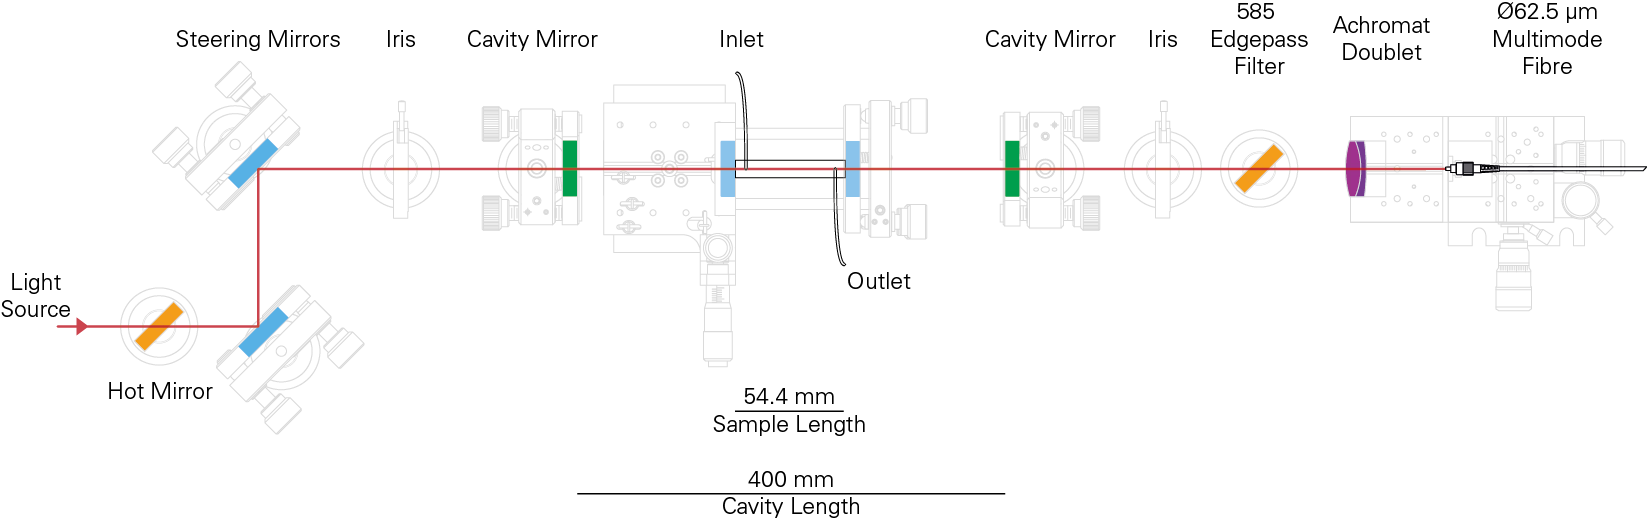
\includegraphics[width=500pt]{figures/bbceas_setup/bbceas_setup.pdf}
\end{center}
\caption{Optical setup for \ac{BBCEAS} experiments performed in this report}
\label{fig:optical_layout}
\end{figure}
\end{wide}


The optical layout for the system used in this report is nearly identical to
all \ac{BBCEAS} layouts \cite{Berden:2009wk}. The light source is a Fianium
\textsc{sc-450} supercontinuum pulsed laser source, with a high enough
repetition rate that it is treated like a continuous wave laser source in our
equations. After the source, an optical cavity is formed with mirrors of
reflectivity $R=0.99$. Finally, light exiting the cavity is coupled into a
multimode fibre and imaged using a custom built grating spectrometer.

Inside the cavity sits a cuvette compressed between two optical windows. This
cuvette holder is then mounted in a rotatable jig to make it easier to properly
align the cuvette with the cavity. This cuvette has inlet and outlet tubes,
which allow for the liquid inside to be changed. This setup was chosen over
mounting the cuvette directly to the mirrors \cite{Seetohul:2009ij} to prevent
the mirrors from accumulating particulates that would add significant noise to
the acquired spectrum.



\section{Potential Enhancements}\label{sec:bbceas_enhance}

While this setup works well, there are certain aspects of the instrument that
can be improved to make either a gain in sensitivity and/or in cost over the
current implementation.

\subsection{LED source}\label{sec:bbceas_led}

\marginpar{See Section~\ref{subsec:led} for a discussion of an \ac{LED} as a light source}

The supercontinuum light source is excellent for its low divergence and high
power properties over the visible range. However, such light sources are far
from cheap, and supercontinuum sources often have high fluctuations in
intensity over time that can be difficult to correct for without a reference
signal.

\acp{LED} offer an enticing visible light source alternative to supercontinuum
sources on the basis of their exceptionally low cost and stable output
intensity stability.

The current costs of high power \ac{LED} devices are on the order of only a few
pounds, and can be easily wired in series with a resistor in order to provide
stable light output. There is a potential complication in the power supplies
for high powered \acp{LED} because of power draw can be quite large.  However,
one can build highly stable current inputs into the \ac{LED} to aid in
stabilising the intensity output \cite{patent_const_current}. Additionally a
thermistor can be added to the \ac{LED} to create a closed loop system, where
the feedback from the thermistor assists in stabilising the light source over
time \cite{Wieman:2000vd}.

Once a stable output intensity is reached, the light from an \ac{LED} can be
fibre coupled into a multimode fibre. The light coming out of the fibre can
then be collimated to create a low divergence beam to be put into the cavity
\cite{Berden:2009wk}.  Other groups have shown that fibre-coupled \ac{LED}
light sources can be used for liquid \ac{BBCEAS} experiments
\cite{Islam:2007ea,Seetohul:2009du}, and that the setup for an \ac{LED} source
is relatively trivial.

An additional benefit of an \ac{LED} based light source is that the intensity
could be easily modulated by an external signal quickly. This could be used to
create lock-in type detection schemes, or to initiate a photochemical reaction
and watch the result through absorption spectroscopy.



\subsection{Non-fibre Spectrometer}\label{subsec:bbceas_no_fibre}

Coupling light into a multimode fibre can provide a convenient way to reroute
light to certain optical setups. The problem with coupling light into a fibre,
even a multimode fibre with a large diameter core, is that the loss of light at
the interface of the fibre is relatively high. Practically, lasers based setups
are unaffected by this coupling problem in \ac{BBCEAS} measurements as it is
often possible to reach higher output power levels with the laser to offset the
coupling losses.  There are even cases where one can saturate the absorber in a
\ac{BBCEAS} measurement if the light intensity is too high
\cite{Giuliano:1967hw}.

Incoherent light sources such as \acp{LED}, on the other hand, suffer from
problems of having wide, divergent emission profiles, which practically means
that these sources have limits on their intensity that cannot offset the fibre
losses. On top of this limit, losses for the incoherent source are higher than
the laser due to the larger spot sizes and diffuse nature of the light when
coupling into a fibre.

The current optical setup is convenient because different detectors can be
easily swapped to provide more accurate or faster acquisitions. But tests with
collimated \ac{LED} light sources in the \ac{BBCEAS} setup used in the report
have required integration times on the order of ten seconds, hampering the
effective use of \ac{LED} sources.

If the light coming out of the cavity is instead directed onto a transmission
grating, the losses due to the coupling would be removed, and much more light
would hit the detector. The loss of convenience would be greatly offset by the
ability acquire data at a faster rate and lower noise than in the case of the
fibre coupled spectrometer.



\subsection{Webcam}\label{subsec:bbceas_webcam}

While the current system uses a \ac{CCD} that costs much less than the
detectors in other \ac{CEAS} and \ac{CRDS} systems, the \ac{CCD} is still on
the order of a thousand pounds to buy at the time of writing. To further reduce
the costs of the \ac{BBCEAS} system, the detector can be replaced with the
\ac{CCD} from a web camera, which costs tens of pounds.

Replacing the \ac{CCD} with a web camera would bring the total costs, if one
uses low reflectivity dielectric mirrors, to potentially less than a hundred
pounds. The \ac{CCD} in a web camera is also incredibly tiny, and would allow
the entire \ac{BBCEAS} setup to be easily miniaturised into a portable device
using an \ac{LED} light source.


\section*{Chapter Review}

\ac{BBCEAS} is a promising new spectroscopic technique that can be utilised to
acquire signals from fiendishly small absorption cross sections. While this
method does contain some error, it can be readily quantified and accounted for
when analysing absorption spectra. While the current implementation of a
\ac{BBCEAS} provides usable results, some enhancements can be made to further
decrease the noise in the acquired signal and increase the intensity of the
light hitting the detector.
